\documentclass{article}\usepackage{graphicx, color}
%% maxwidth is the original width if it is less than linewidth
%% otherwise use linewidth (to make sure the graphics do not exceed the margin)
\makeatletter
\def\maxwidth{ %
  \ifdim\Gin@nat@width>\linewidth
    \linewidth
  \else
    \Gin@nat@width
  \fi
}
\makeatother

\definecolor{fgcolor}{rgb}{0.2, 0.2, 0.2}
\newcommand{\hlnumber}[1]{\textcolor[rgb]{0,0,0}{#1}}%
\newcommand{\hlfunctioncall}[1]{\textcolor[rgb]{0.501960784313725,0,0.329411764705882}{\textbf{#1}}}%
\newcommand{\hlstring}[1]{\textcolor[rgb]{0.6,0.6,1}{#1}}%
\newcommand{\hlkeyword}[1]{\textcolor[rgb]{0,0,0}{\textbf{#1}}}%
\newcommand{\hlargument}[1]{\textcolor[rgb]{0.690196078431373,0.250980392156863,0.0196078431372549}{#1}}%
\newcommand{\hlcomment}[1]{\textcolor[rgb]{0.180392156862745,0.6,0.341176470588235}{#1}}%
\newcommand{\hlroxygencomment}[1]{\textcolor[rgb]{0.43921568627451,0.47843137254902,0.701960784313725}{#1}}%
\newcommand{\hlformalargs}[1]{\textcolor[rgb]{0.690196078431373,0.250980392156863,0.0196078431372549}{#1}}%
\newcommand{\hleqformalargs}[1]{\textcolor[rgb]{0.690196078431373,0.250980392156863,0.0196078431372549}{#1}}%
\newcommand{\hlassignement}[1]{\textcolor[rgb]{0,0,0}{\textbf{#1}}}%
\newcommand{\hlpackage}[1]{\textcolor[rgb]{0.588235294117647,0.709803921568627,0.145098039215686}{#1}}%
\newcommand{\hlslot}[1]{\textit{#1}}%
\newcommand{\hlsymbol}[1]{\textcolor[rgb]{0,0,0}{#1}}%
\newcommand{\hlprompt}[1]{\textcolor[rgb]{0.2,0.2,0.2}{#1}}%

\usepackage{framed}
\makeatletter
\newenvironment{kframe}{%
 \def\at@end@of@kframe{}%
 \ifinner\ifhmode%
  \def\at@end@of@kframe{\end{minipage}}%
  \begin{minipage}{\columnwidth}%
 \fi\fi%
 \def\FrameCommand##1{\hskip\@totalleftmargin \hskip-\fboxsep
 \colorbox{shadecolor}{##1}\hskip-\fboxsep
     % There is no \\@totalrightmargin, so:
     \hskip-\linewidth \hskip-\@totalleftmargin \hskip\columnwidth}%
 \MakeFramed {\advance\hsize-\width
   \@totalleftmargin\z@ \linewidth\hsize
   \@setminipage}}%
 {\par\unskip\endMakeFramed%
 \at@end@of@kframe}
\makeatother

\definecolor{shadecolor}{rgb}{.97, .97, .97}
\definecolor{messagecolor}{rgb}{0, 0, 0}
\definecolor{warningcolor}{rgb}{1, 0, 1}
\definecolor{errorcolor}{rgb}{1, 0, 0}
\newenvironment{knitrout}{}{} % an empty environment to be redefined in TeX

\usepackage{alltt}
\usepackage{hyperref}
\title{Notes for Week 2}
\author{Rob Hayward}
\IfFileExists{upquote.sty}{\usepackage{upquote}}{}
\begin{document}
\maketitle

\section{Control structures}
The are a number of structures that can be used. 
\begin{knitrout}
\definecolor{shadecolor}{rgb}{0.969, 0.969, 0.969}\color{fgcolor}\begin{kframe}
\begin{alltt}
\hlfunctioncall{if}(<condition>) \{
\hlcomment{  ## do something}
\} else \{
\hlcomment{  ## do something else}
\}
\end{alltt}
\end{kframe}
\end{knitrout}

The loop structure.
\begin{knitrout}
\definecolor{shadecolor}{rgb}{0.969, 0.969, 0.969}\color{fgcolor}\begin{kframe}
\begin{alltt}
\hlfunctioncall{for} (i in 1:10) \{
    \hlfunctioncall{print}(i)
\}
\end{alltt}
\end{kframe}
\end{knitrout}

While 
\begin{knitrout}
\definecolor{shadecolor}{rgb}{0.969, 0.969, 0.969}\color{fgcolor}\begin{kframe}
\begin{alltt}
count <- 0
\hlfunctioncall{while} (count < 10) \{
    \hlfunctioncall{print}(count)
    count <- count + 1
\}
\end{alltt}
\end{kframe}
\end{knitrout}

Example using the logical operator. 
\begin{knitrout}
\definecolor{shadecolor}{rgb}{0.969, 0.969, 0.969}\color{fgcolor}\begin{kframe}
\begin{alltt}
z = 5
\hlfunctioncall{while} (z >= 3 && z <= 10) \{
    \hlfunctioncall{print}(z)
    coin <- \hlfunctioncall{rbinom}(1, 1, 0.5)
    \hlfunctioncall{if} (coin == 1) \{
\hlcomment{        # random walk}
        z <- z + 1
    \} else \{
        z <- z - 1
    \}
\}
\end{alltt}
\end{kframe}
\end{knitrout}

Repeat can be used with break. 
\begin{knitrout}
\definecolor{shadecolor}{rgb}{0.969, 0.969, 0.969}\color{fgcolor}\begin{kframe}
\begin{alltt}
x0 <- 1
tol <- 1e-08

repeat \{
    x1 <- \hlfunctioncall{computeEstimate}()
    \hlfunctioncall{if} (\hlfunctioncall{abs}(x1 - x0) <= tol) \{
        break
    \} else \{
        x0 <- x1
    \}
\}
\end{alltt}
\end{kframe}
\end{knitrout}

This is often used in an optimisation algorithm. However, it is Usually better to use a for loop with a set length so that there is a break and you avoid an infinite loop. 
\begin{knitrout}
\definecolor{shadecolor}{rgb}{0.969, 0.969, 0.969}\color{fgcolor}\begin{kframe}
\begin{alltt}
\hlfunctioncall{for} (i in 1:10) \{
    \hlfunctioncall{if} (i <= 20) \{
\hlcomment{        ## skip the first 20 iterations}
        next
    \}
\hlcomment{    ## do something here}
\}
\end{alltt}
\end{kframe}
\end{knitrout}

Does not use the first 20 attempts. 

\section{Functions}
The basic style is 
\begin{knitrout}
\definecolor{shadecolor}{rgb}{0.969, 0.969, 0.969}\color{fgcolor}\begin{kframe}
\begin{alltt}
x <- \hlfunctioncall{function}(<arguments>)\{
\hlcomment{  ## do something interesting}
\}
\end{alltt}
\end{kframe}
\end{knitrout}

Functions are \emph{first class objects}.  They can be passed on and nested inside another function.  The last expression is returned.  Formals will return a list of all the formal arguments in a function. Arguments can be matched by position or name. Lazy evaluation means that arguments are only evaluated when they are needed. This prevent errors happening easiy. It is posible to use \dots to pass a function that you do not want to repeat.  For example, if you were to create a version of plot, it is possible to do the following
\begin{knitrout}
\definecolor{shadecolor}{rgb}{0.969, 0.969, 0.969}\color{fgcolor}\begin{kframe}
\begin{alltt}
myplot <- \hlfunctioncall{function}(x, y, type = \hlstring{"l"}, ...) \{
    \hlfunctioncall{plot}(x, y, type = type, ...)
\}
\end{alltt}
\end{kframe}
\end{knitrout}

The \dots can also be used when dealing with \emph{generic functions}.  These are functions that dispatch methods to different types of data.  More on this later.  The \dots can also be used when the arguments are not known in advance. For example, the \emph{paste} function uses this because it is possible to push as many strings as possible.  Anything after \dots must be named explicitly. 

One issue that emerges is how does R know what to do if I assign a symbol that is already attatched to a function to a new function.  For example, what happens if I assign something to lm?  R needs to bind a value to the symbol.  In this case it is a function that is bound to the lm symbol. R looks through the various \emph{environment}.  It first looks in the \emph{Global Environment}. Therefore, if you assign something it is in the Global Environment.  It will look through the list of Environments until it finds a match.  The base package is always the last.  The order of the packages matters.  If library() is used to load package, it is placed behind the Global Environment (second in the list).  It is possible to have different objects with the same symbol.  For example, there could be a function called \emph{c} and a vector called \emph{c}. 

\section{Scoping Rules}
The scoping rules determine how a value is associated with a free variable in a function.  R uses lexical scoping or static scoping rather than dynamic scoping. Free variables are those that are not formal arguments and not local variables (those that are assigned inside the function body).  The values of free variables are searched for in the environment in which the function was defined. An environment is a collection of symbol-value pairs (x is the symbol and 2.3 may be its value).  Every environment (collection of symbol-value paris) has a partent environment and an environment may have a number of children. Once a function is associated with an environment, there is \emph{closure} or \emph{environment closure}.  

R will look in the environment that the function was defined if it cannot find a value in the function.  If it cannot find it there, it will look in the parent environment.  It will continue looking down the list of environments until it comes to the Globa Environment. It wll continue until it gets to the empty
environment and then throw an error. 

Typlically, the function is defined in the global environment.  This is what is usual and the response is expected.  However, sometimes it is possible to return a function from a function.  In this case, the function has been defined in the fucntion not the global environment.  These are often of a sort of \emph{constructor functions}.  The function is constructing another function. For example, 
\begin{knitrout}
\definecolor{shadecolor}{rgb}{0.969, 0.969, 0.969}\color{fgcolor}\begin{kframe}
\begin{alltt}
make.power <- \hlfunctioncall{function}(n) \{
    pow <- \hlfunctioncall{function}(x) \{
        x^n
    \}
    pow
\}
\end{alltt}
\end{kframe}
\end{knitrout}

The function pow is returned.  n is a free variable.  It is defined in the pow function.  
\begin{knitrout}
\definecolor{shadecolor}{rgb}{0.969, 0.969, 0.969}\color{fgcolor}\begin{kframe}
\begin{alltt}
cube <- \hlfunctioncall{make.power}(3)
square <- \hlfunctioncall{make.power}(2)
\hlfunctioncall{cube}(3)
\end{alltt}
\begin{verbatim}
## [1] 27
\end{verbatim}
\begin{alltt}
\hlfunctioncall{square}(3)
\end{alltt}
\begin{verbatim}
## [1] 9
\end{verbatim}
\end{kframe}
\end{knitrout}

it is possible to look into the environment 
\begin{knitrout}
\definecolor{shadecolor}{rgb}{0.969, 0.969, 0.969}\color{fgcolor}\begin{kframe}
\begin{alltt}
\hlfunctioncall{ls}(\hlfunctioncall{environment}(cube))
\end{alltt}
\begin{verbatim}
## [1] "n"   "pow"
\end{verbatim}
\begin{alltt}
\hlfunctioncall{get}(\hlstring{"n"}, \hlfunctioncall{environment}(cube))
\end{alltt}
\begin{verbatim}
## [1] 3
\end{verbatim}
\end{kframe}
\end{knitrout}

R looks for the value of free variable in the \emph{defining} environment.  In dynamic scoping, the programe looks for the free variable in the \emph{calling} environment. This means that all objects have to be stored in memory. All functions must have a pointer to its defining environment.  This can be complex becaus there can be functions within functions. 

This is important because it will facilitate optimisation. There are a number of optimisation functions in R such as \emph{optim}, \emph{nlm} and \emph{optimize}.  They all require functions be passed to the function where the arguments are the vector parameters. The aim is to create a constructor function which \emph{construts} the objective function.  All the data and all the things that the objective function depends on will be included in the defining environment. For example, 
\begin{knitrout}
\definecolor{shadecolor}{rgb}{0.969, 0.969, 0.969}\color{fgcolor}\begin{kframe}
\begin{alltt}
make.NetLogLik <- \hlfunctioncall{function}(data, fixed = \hlfunctioncall{c}(FALSE, FALSE)) \{
    params <- fixed
    \hlfunctioncall{function}(p) \{
        params[!fixed] <- p
        mu <- params[1]
        sigma <- params[2]
        a <- -0.5 * \hlfunctioncall{length}(data) * \hlfunctioncall{log}(2 * pi * sigma^2)
        b <- -0.5 * \hlfunctioncall{sum}((data - mu)^2)/(sigma^2)
        -(a + b)
    \}
\}
\end{alltt}
\end{kframe}
\end{knitrout}

This is a log likelihood function that depends on the data and a logical vector that will allow some of the parameters to be fixed.  Inside the constructor function, another function is defined that will optimise over the mean and the standard deviation. The constructor function returns the function as the return value. 
\begin{knitrout}
\definecolor{shadecolor}{rgb}{0.969, 0.969, 0.969}\color{fgcolor}\begin{kframe}
\begin{alltt}
\hlfunctioncall{set.seed}(1)
normals <- \hlfunctioncall{rnorm}(100, 1, 2)
nLL <- \hlfunctioncall{make.NetLogLik}(normals)
nLL
\end{alltt}
\begin{verbatim}
## function(p) {
##         params[!fixed] <- p
##         mu <- params[1]
##         sigma <- params[2]
##         a <- -0.5 * length(data) * log(2 * pi * sigma^2)
##         b <- -0.5 * sum((data - mu)^2)/(sigma^2)
##         -(a + b)
##     }
## <environment: 0x000000000707cd28>
\end{verbatim}
\begin{alltt}
\hlfunctioncall{ls}(\hlfunctioncall{environment}(nLL))
\end{alltt}
\begin{verbatim}
## [1] "data"   "fixed"  "params"
\end{verbatim}
\end{kframe}
\end{knitrout}

The address of the environment that the function is in is returned. "Data" is a free variable (not a formal or informal argument). The data has to be looked up in the environment where the data was defined.  If you look at this environment by calling ls(), you will see the free variable that are defined in the defining environment.  

Now optim() can be called on the fuction. 
\begin{knitrout}
\definecolor{shadecolor}{rgb}{0.969, 0.969, 0.969}\color{fgcolor}\begin{kframe}
\begin{alltt}
\hlfunctioncall{optim}(\hlfunctioncall{c}(mu = 0, sigma = 1), nLL)$par
\end{alltt}
\begin{verbatim}
##    mu sigma 
## 1.218 1.787
\end{verbatim}
\end{kframe}
\end{knitrout}

The estimates of the mean and sigma are pretty accurate.  Alternatively, it is possible to fix sigma at its actual value and estimate the mean.  First, re-set the negative log likelihood function. 
\begin{knitrout}
\definecolor{shadecolor}{rgb}{0.969, 0.969, 0.969}\color{fgcolor}\begin{kframe}
\begin{alltt}
nLL <- \hlfunctioncall{make.NetLogLik}(normals, \hlfunctioncall{c}(FALSE, 2))
\hlfunctioncall{optimize}(nLL, \hlfunctioncall{c}(1e-06, 10))$minimum
\end{alltt}
\begin{verbatim}
## [1] 1.218
\end{verbatim}
\end{kframe}
\end{knitrout}

The log likeihood can also be plotted.  Create a sequence of x values and apply those to the nLL function (with the mean fixed at 1) and plot the result for the standard deviation.  
\begin{knitrout}
\definecolor{shadecolor}{rgb}{0.969, 0.969, 0.969}\color{fgcolor}\begin{kframe}
\begin{alltt}
nLL <- \hlfunctioncall{make.NetLogLik}(normals, \hlfunctioncall{c}(1, FALSE))
x <- \hlfunctioncall{seq}(1.7, 1.9, length = 100)
y <- \hlfunctioncall{sapply}(x, nLL)
\hlfunctioncall{plot}(x, \hlfunctioncall{exp}(-(y - \hlfunctioncall{min}(y))), type = \hlstring{"l"}, main = \hlstring{"NLL and values of SD"})
\end{alltt}
\end{kframe}
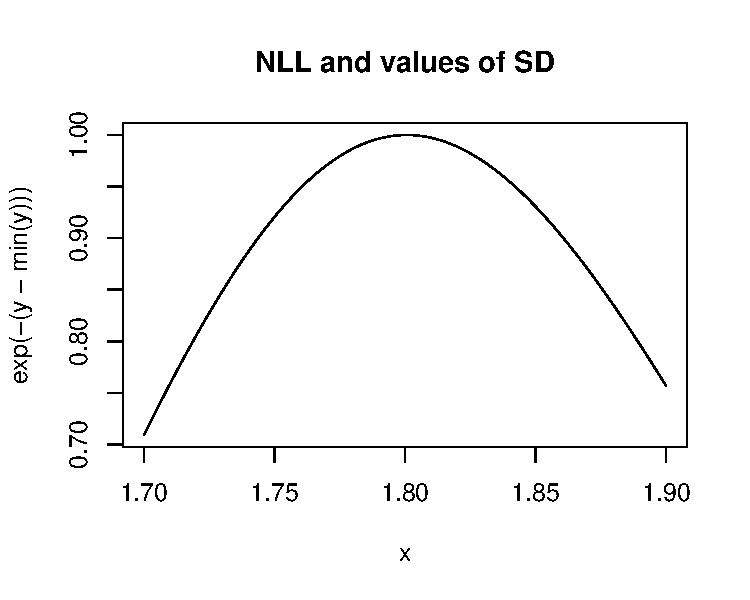
\includegraphics[width=\maxwidth]{figure/plotllsd} 

\end{knitrout}

Similarly for the mean. 
\begin{knitrout}
\definecolor{shadecolor}{rgb}{0.969, 0.969, 0.969}\color{fgcolor}\begin{kframe}
\begin{alltt}
nLL <- \hlfunctioncall{make.NetLogLik}(normals, \hlfunctioncall{c}(FALSE, 2))
x <- \hlfunctioncall{seq}(0.5, 1.5, length = 100)
y <- \hlfunctioncall{sapply}(x, nLL)
\hlfunctioncall{plot}(x, \hlfunctioncall{exp}(-(y - \hlfunctioncall{min}(y))), type = \hlstring{"l"}, main = \hlstring{"NLL and values of mean"})
\end{alltt}
\end{kframe}
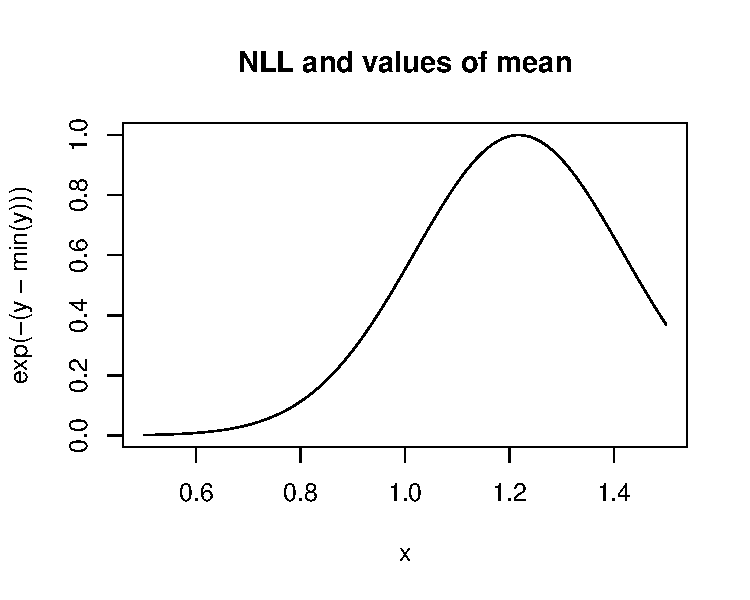
\includegraphics[width=\maxwidth]{figure/plotllm} 

\end{knitrout}


\section{Loop functions}
The main loop functions are lapply, sapply apply, tapply, mapply. There is also the function split that will split things into small items. lapply will also return a list.  The function will apply a function to each element of the list. the \dots can be used to send arguments to the functiont that is being applied. 

There is a lot of use of \emph{anonymous functions}.  An an anonymous function is one that is made on the fly.  For example, to extract the first column, 
\begin{knitrout}
\definecolor{shadecolor}{rgb}{0.969, 0.969, 0.969}\color{fgcolor}\begin{kframe}
\begin{alltt}
x = \hlfunctioncall{list}(a = \hlfunctioncall{matrix}(1:4, 2, 2), b <- \hlfunctioncall{matrix}(1:6, 3, 2))
x
\end{alltt}
\begin{verbatim}
## $a
##      [,1] [,2]
## [1,]    1    3
## [2,]    2    4
## 
## [[2]]
##      [,1] [,2]
## [1,]    1    4
## [2,]    2    5
## [3,]    3    6
\end{verbatim}
\begin{alltt}
\hlfunctioncall{lapply}(x, \hlfunctioncall{function}(elt) elt[, 1])
\end{alltt}
\begin{verbatim}
## $a
## [1] 1 2
## 
## [[2]]
## [1] 1 2 3
\end{verbatim}
\end{kframe}
\end{knitrout}

The function to extract the column has to be made up on the spot. 

sapply will try to simplify the result of lapply.  It can change a list into a vector or matrix if it is more appropriate (where each element has a length of onme or there are seveal elements of the same length).  For example, 
\begin{knitrout}
\definecolor{shadecolor}{rgb}{0.969, 0.969, 0.969}\color{fgcolor}\begin{kframe}
\begin{alltt}
x <- \hlfunctioncall{list}(\hlfunctioncall{rnorm}(100), \hlfunctioncall{runif}(100), \hlfunctioncall{rpois}(100, 1))
\hlfunctioncall{sapply}(x, quantile, probs = \hlfunctioncall{c}(0.25, 0.75))
\end{alltt}
\begin{verbatim}
##        [,1]   [,2] [,3]
## 25% -0.6510 0.2557    0
## 75%  0.5009 0.7655    2
\end{verbatim}
\end{kframe}
\end{knitrout}

Apply is the same sort of function that works on arrays.  A matrix is the simplest form of arrays. The \emph{margin} is the dimension over which the function is to be appled.  Dimension 1 applies to rows, dimension 2 is the columns.  
\begin{knitrout}
\definecolor{shadecolor}{rgb}{0.969, 0.969, 0.969}\color{fgcolor}\begin{kframe}
\begin{alltt}
x <- \hlfunctioncall{matrix}(\hlfunctioncall{rnorm}(200), 20, 20)
\hlfunctioncall{apply}(x, 2, mean)
\end{alltt}
\begin{verbatim}
##  [1]  0.21051  0.09443  0.02218 -0.15933  0.09021  0.14723 -0.22431
##  [8] -0.49658  0.30095  0.07704  0.21051  0.09443  0.02218 -0.15933
## [15]  0.09021  0.14723 -0.22431 -0.49658  0.30095  0.07704
\end{verbatim}
\end{kframe}
\end{knitrout}

There are other functions that are optimised to work more swiftly. 
\begin{itemize}
\item rowSums = apply(x, 1, sum)
\item rowMeans = apply(x, 1, mean)
\item colSums = apply(x, 2, sum)
\item colMeans = apply(x, 2, mean)
\end{itemize}
If you want to apply a function across an array with more than two dimensions, identify the dimensions that are to be preserved.  For example, if there is an array of 2 by 2 matrices, to take the mean of the row and columns of all of them.
\begin{knitrout}
\definecolor{shadecolor}{rgb}{0.969, 0.969, 0.969}\color{fgcolor}\begin{kframe}
\begin{alltt}
a <- \hlfunctioncall{array}(\hlfunctioncall{rnorm}(2 * 2 * 10), \hlfunctioncall{c}(2, 2, 10))
\hlfunctioncall{apply}(a, \hlfunctioncall{c}(1, 2), mean)
\end{alltt}
\begin{verbatim}
##         [,1]    [,2]
## [1,] 0.11176 -0.5831
## [2,] 0.01838  0.1728
\end{verbatim}
\end{kframe}
\end{knitrout}

This will return the mean of the rows and the mean of the columns.  

tapply will apply some function to a subset of the vector.  the Index argument will determine which parts of the vector or matrix will be assessed. It should be a list of factors or something that can be coerced into a factor. The result can be simplified (default is TRUE). For example, if 30 variables are created and factors are allocated, the mean by factor can be calculated. 
\begin{knitrout}
\definecolor{shadecolor}{rgb}{0.969, 0.969, 0.969}\color{fgcolor}\begin{kframe}
\begin{alltt}
x <- \hlfunctioncall{c}(\hlfunctioncall{rnorm}(10), \hlfunctioncall{runif}(10), \hlfunctioncall{rnorm}(10, 1))
f <- \hlfunctioncall{gl}(3, 10)
\hlfunctioncall{tapply}(x, f, mean)
\end{alltt}
\begin{verbatim}
##        1        2        3 
## -0.02514  0.43427  0.49939
\end{verbatim}
\end{kframe}
\end{knitrout}

If you do not simplify the result, you will get a list back. 

tapply is useful because it splits the matrix and then puts it back together.  The split() function takes a vector and a factor variable and splits the vector into the number of groups implied by the factors.  Split will always return a list. This is more or less what tapply does.  However, the split function can be applied to much more complicated objects.  For example, to calculate mean temerature for each month in the following dataframe.  
\begin{knitrout}
\definecolor{shadecolor}{rgb}{0.969, 0.969, 0.969}\color{fgcolor}\begin{kframe}
\begin{alltt}
\hlfunctioncall{library}(datasets)
\hlfunctioncall{head}(airquality)
\end{alltt}
\begin{verbatim}
##   Ozone Solar.R Wind Temp Month Day
## 1    41     190  7.4   67     5   1
## 2    36     118  8.0   72     5   2
## 3    12     149 12.6   74     5   3
## 4    18     313 11.5   62     5   4
## 5    NA      NA 14.3   56     5   5
## 6    28      NA 14.9   66     5   6
\end{verbatim}
\begin{alltt}
s <- \hlfunctioncall{split}(airquality, airquality$Month)
\hlfunctioncall{sapply}(s, \hlfunctioncall{function}(x) \hlfunctioncall{colMeans}(x[, \hlfunctioncall{c}(\hlstring{"Ozone"}, \hlstring{"Solar.R"}, \hlstring{"Wind"})], na.rm = TRUE))
\end{alltt}
\begin{verbatim}
##              5      6       7       8      9
## Ozone    23.62  29.44  59.115  59.962  31.45
## Solar.R 181.30 190.17 216.484 171.857 167.43
## Wind     11.62  10.27   8.942   8.794  10.18
\end{verbatim}
\end{kframe}
\end{knitrout}

Using the sapply function will ensure that a matrix is returned rather than a lsit.  The na.rm = TRUE allows the mean() function to be evaluated. 

It is also possible to split over more than one level.  If there is more than one factor. For example, here two factors are created, one with two levels (f1) and one with five levels (f2).  This means that there are 10 possible combinations.  
\begin{knitrout}
\definecolor{shadecolor}{rgb}{0.969, 0.969, 0.969}\color{fgcolor}\begin{kframe}
\begin{alltt}
x <- \hlfunctioncall{rnorm}(10)
f1 <- \hlfunctioncall{gl}(2, 5)
f2 <- \hlfunctioncall{gl}(5, 2)
\hlfunctioncall{interaction}(f1, f2)
\end{alltt}
\begin{verbatim}
##  [1] 1.1 1.1 1.2 1.2 1.3 2.3 2.4 2.4 2.5 2.5
## Levels: 1.1 2.1 1.2 2.2 1.3 2.3 1.4 2.4 1.5 2.5
\end{verbatim}
\begin{alltt}
\hlfunctioncall{str}(\hlfunctioncall{split}(x, \hlfunctioncall{list}(f1, f2), drop = TRUE))
\end{alltt}
\begin{verbatim}
## List of 6
##  $ 1.1: num [1:2] 1.097 -0.248
##  $ 1.2: num [1:2] -0.16 -0.626
##  $ 1.3: num 0.9
##  $ 2.3: num -0.994
##  $ 2.4: num [1:2] 0.849 0.806
##  $ 2.5: num [1:2] -0.468 0.848
\end{verbatim}
\end{kframe}
\end{knitrout}

Drop = TRUE will get rid of the new combined factors (10) that do not have any members. 

\end{document}
